\documentclass[specification,annotation,times]{itmo-student-thesis}

%% Опции пакета:
%% - specification - если есть, генерируется задание, иначе не генерируется
%% - annotation - если есть, генерируется аннотация, иначе не генерируется
%% - times - делает все шрифтом Times New Roman, требует пакета pscyr.

%% Данные пакеты необязательны к использованию в бакалаврских/магистерских
%% Они нужны для иллюстративных целей

%% Начало
\usepackage{tikz}
\usetikzlibrary{arrows}
\usepackage{filecontents}
\begin{filecontents}{master-thesis.bib}
@inproceedings{ example-english,
    year        = {2015},
    booktitle   = {Proceedings of IEEE Congress on Evolutionary Computation},
    author      = {Maxim Buzdalov and Anatoly Shalyto},
    title       = {Hard Test Generation for Augmenting Path Maximum Flow 
                   Algorithms using Genetic Algorithms: Revisited},
    pages       = {2121-2128},
    langid      = {english}
}

@article{ example-russian,
    author      = {Максим Викторович Буздалов},
    title       = {Генерация тестов для олимпиадных задач по программированию 
                   с использованием генетических алгоритмов},
    journal     = {Научно-технический вестник {СПбГУ} {ИТМО}},
    number      = {2(72)},
    year        = {2011},
    pages       = {72-77},
    langid      = {russian}
}

@article{ unrestricted-jump-evco,
    author      = {Maxim Buzdalov and Benjamin Doerr and Mikhail Kever},
    title       = {The Unrestricted Black-Box Complexity of Jump Functions},
    journal     = {Evolutionary Computation},
    year        = {2016},
    note        = {Accepted for publication},
    langid      = {english}
}

\end{filecontents}
%% Конец

%% Указываем файл с библиографией.
\addbibresource{master-thesis.bib}

\begin{document}

\studygroup{M4239}
\title{Верхние и нижние оценки несмещенной вычислительной сложности оптимизационной задачи Needle}
\author{Волочай Виктория Олеговна}{Волочай В.О.}
\supervisor{Буздалов Максим Викторович}{Буздалов М.В.}{канд. техн. наук}{доцент кафедры компьютерных технологий Университета ИТМО}
\publishyear{2016}
%% Дата выдачи задания. Можно не указывать, тогда надо будет заполнить от руки.
%\startdate{01}{сентября}{2013}
%% Срок сдачи студентом работы. Можно не указывать, тогда надо будет заполнить от руки.
%\finishdate{31}{мая}{2015}
%% Дата защиты. Можно не указывать, тогда надо будет заполнить от руки.
\defencedate{21}{июня}{2016}

%\addconsultant{}{}
%\addconsultant{}{}

%% Задание
%%% Техническое задание и исходные данные к работе
\technicalspec{Необходимо рассмотреть алгоритм решения задачи оптимизационной задачи Needle, применив к задаче модификации, основанные на идеях black-box сложности. Соответственно, необходимо оценить время работы алгоритмов, использующих для решения несмещенные операторы, таким образом получив верхние и нижние оценки.}

%%% Содержание выпускной квалификационной работы (перечень подлежащих разработке вопросов)
\plannedcontents{Работа должна содержать обзор предметной области, в частности, описания задачи Needle, black-box сложности, модели несмещенной сложности и несмещенных операторов. Так же основная часть работы должна представлять собой описание применения black-box оптимизации к задаче и её решений с использованием несмещенных операторов. Результатом работы должны быть оценки времени работы конкретного алгоритма, решающего задачу, являющиеся верхними оценками, а так же нижние оценки на сложность работы алгоритмов на данном классе задач.}

%%% Исходные материалы и пособия 
\plannedsources{\begin{enumerate}
    \item B. Doerr and C. Winzen. Reducing the arity in unbiased black-box complexity. Theor. Comput. Sci., 545:108–121, 2014;
    \item Stefan Droste, Thomas Jansen, and Ingo Wegener. Upper and lower bounds for randomized search heuristics in black-box optimization. Theory of Computing Systems, 39:525–544, 2006
    \item Per Kristian Lehre and Carsten Witt. Black-box search by unbiased variation. In Proceedings of Genetic and Evolutionary Computation Conference (GECCO’10), pages 1441– 1448. ACM, 2010.
\end{enumerate}}

%%% Календарный план
\addstage{Ознакомление с оптимизационной задачей Needle}{12.2014}
\addstage{Ознакомление с black-box сложностью и несмещенной моделью}{12.2014}
\addstage{Исследование алгоритмов решения задачи с применением несмещенных операторов арностей k = 1, 2, 3}{09.2015}
\addstage{Моделирование работы алгоритмов}{11.2015}
\addstage{Написание пояснительной записки}{03.2016}

%%% Цель исследования
\researchaim{Нахождение верхних и нижних оценок времени работы алгоритмов, решающих задачу Needle с помощью несмещенных операторов.}

%%% Задачи, решаемые в ВКР
\researchtargets{\begin{enumerate}
    \item Рассмотрение задачи Needle в несмещенной модели. 
    \item Нахождение верхних и нижних оценок для алгоритмов арностей k = 1, 2, 3;
\end{enumerate}}


%%% Использование современных пакетов компьютерных программ и технологий
\advancedtechnologyusage{Для
реализации алгоритмов и оценки времени работы был использован язык программирования Python, а так же библиотеки Numpy и Matplotlib, использованные для анализа алгоритмов и построения графиков. В качестве сред для разработки использовались PyCharm и Spyder. Для написания пояснительной записки было использовано издательское ПО \LaTex.}

%%% Краткая характеристика полученных результатов 
\researchsummary{Были найдены верхние оценки для
несмещенных операторов арностей 1, 2, 3, решающих задачу Needle. Было установлено, что верхняя и нижняя оценка времени работы тернарного оператора совпадают.}

%%% Гранты, полученные при выполнении работы 
\researchfunding{Нет.}

%%% Наличие публикаций и выступлений на конференциях по теме выпускной работы
\researchpublications{По теме этой работы были выступения на следующих конференциях
\begin{enumerate}
    \item Конференция молодых ученых 2016
    \item Конференция СПИСОК 2016
\end{enumerate}
По результатам конференций будут выпущены сборники с материалами работы.
}

%% Эта команда генерирует титульный лист и аннотацию.
\maketitle{Магистр}

%% Оглавление
\tableofcontents

%% Макрос для введения. Совместим со старым стилевиком.


\startthechapters
\startprefacepage

Одним из способов применения эволюционных алгоритмов является решение оптимизационных задач. Одной из таких задач является задача Needle. Для получения улучшенных оценок сложности работы алгоритма, рассмотрим задачу в модификации, основанной на идеях black-box сложности.  


% как-то добавить и переформулировать
  Модель непредвзятый черного ящика введена в Lehre и Уитт (2012) является в настоящее время одним из стандартные модели сложности в эволюционных вычислениях. В частности, унарным непредвзятый модель дает более реалистичную оценку сложности для ряда функций, чем исходного неограниченного черного ящика модели Droste и др. (2006). Важным преимуществом несмещенной модели является то, что она позволяет нам анализировать влияние арностью операторов выборки в использовании. Кроме того, новые точки поиска могут быть выбраны либо только равномерно случайным образом или из распределений, которые зависят от ранее созданных точек поиска непредвзято. В этом разделе мы дадим краткое определение модели черного ящика беспристрастной, указывая на Lehre и Уитт (2012) и Doerr и Winzen (2014b) для более подробного введения
  
  
\chapter{Обзор предметной области}
\label{chapter1}

В этой главе приводится описание работы, обзор предметной области, основные термины, встречающиеся в тексте. Основная задача этой главы - изложение теории вычислительной сложности из которой вытекает описание алгоритма черного ящика, а так же black-box сложности с её моделями, особенно акцентируя внимания на несмещенной модели.

\section{Теория сложности эволюционных вычислений}
Рандомизированный поиск эвристик является одним из основных подходов для решения задач оптимизации. Практическим путем было установлено, что рандомизированный подход
часто является довольно успешным, и таким образом широко используется. Его основное преимущество заключается в том, что нет необходимости в глубоком понимании самой
оптимизационной задачи, и полученные походы после легко могут быть повторно переиспользованы на аналогичных задачах.

Одна из проблем таких эвристик заключается в том, что трудно предсказать, какая из задач легкоразрешима поиском рандомизированных эвристик, а какая трудно. Тем не менее, для понимания того, 
какие задачи легкие, а какие трудные, была весьма необходима теория сложности похожая на то, что существует в классической алгоритмике. Таким образом, модель black-box сложности была первой 
попыткой ввести подобную теорию сложности была представлена в работе~\cite{2}. 

Было установлено, что для многих задач наилучший black-box алгоритм работает быстрее, чем существующие эволюционные подходы (к примеру, алгоритм $(1+1)$, который оптимизирует гораздо медленнее). 
Таким образом, одна из целей работы~--- рассмотреть классы алгоритмов с несмещенными~\cite{6} операторами различных арностей: unary (мутации), binary (кроссовер) и~т.д.

\subsection{Black-box сложность}

В этой части определена одна из моделей и black-box сложности, а именно несмещенная модель.
Black-box сложность изучает, сколько оценок функции необходимо при ожидании, пока оптимальный алгоритм черного ящика первый раз вернет оптимальное решение задачи.
Как правило, рандомизированные алгоритмы поиска эвристики, как и эволюционные алгоритмы, являются подобными оптимизаторами с черным ящиком: они чаще всего не зависят
от задачи и, как таковые, узнают о задаче только когда она решена путем создания и оценки точек множества поиска.

Оценка black-box сложности задачи обычно является оценкой фитнес-функции, необходимой для любой поисковой эвристики для решения задачи.

Существует несколько моделей black-box сложности: неограниченная, несмещенная, компараторная b т.д. Неограниченная модель никак не ограничевает никаким образом процедуру отбора и выбора алгоритмов, можно использовать любой алгоритм, работающий с экземпляром как с черным ящиком. В компараторной модели значения функции можно только сравнивать, а сами значения использовать нельзя. А так же существует несмещенная модель, в которой можно использовать алгоритм, манипулирующий с запросами с помощью только несмещенных операторов, которые будут формально определены в работе позднее. В основном, множество эволюционных алгоритмов несмещенные (за исключением некоторых операторов кроссовера). Так же алгоритм не должен различать значения $0/1$ и индексы битов.

\subsection{Несмещенная black-box сложность}
Как уже упоминалось, некоторые недостатки неограниченной black-box модели вдохновили Лехре и Витт~\cite{1} на то, чтобы ввести новую, модель черного ящика c более ограничительным характером, как и 
появилась несмещенная black-box модель. Она остнована на наблюдении, что многие рандомизированные алгоритмы поиска эвристики используют только несмещенные операторы вариаций. 
В этой части будет кратко представлена несмещенная black-box модель. 

Несмещенная модель black-box сложности  представляет собой особый интерес в рамках данной работы. Модель определяет класс aлгoритмoв. Таким образом, сложность класса определяется относительно алгоритмов
в представленной модели.

Пусть существует некоторый класс функций $F$, который известен алгоритму. Возьмем некоторую функцию $f$, такую что $f \in F$, и скрываем от алгоритма. Алгоритм может получать информацию о функции 
только с помощью запросов к черному ящику о значениях $f$ в некоторых точках пространства поиска. Задача алгоритма заключается в том, чтобы найти некий глобальный оптимум функции.

%Формально определим black-box сложность. Мы будем
%оценивать исключительно число запросов к оракулу, считая все %остальные вычисления бесплатными. Время работы TA,f вероятностного %алгоритма A для функции f — это ожидаемое число запросов до момента %нахождения точки оптимума.


\begin{definition}
(Несмещенный оператор арности $k$~\cite{1}). Возьмем некоторое $k \in  N$ и зафиксируем. Несмещенным распределением арности $k$ $D(\cdot | x^{1}, ..., x^k)$  называется такое вероятностое распределение 
над $\{0, 1\}^{n}$, что для любых $y,z \in \{0, 1 \}^n$ и перестановки $\sigma$ и размера $n$ выполняются следующие два условия:
\begin{enumerate}
\item $D ( y | x^{1},..., x^{k} ) = D(\sigma(y) | \sigma(x^{1}),...., \sigma(x^{k}))$;
\item $D ( y | x^{1},..., x^{k} ) = D(y \oplus z | x^{1} \oplus z,...., x^{k} \oplus z)$. 
\end{enumerate}
\end{definition}

Первое свойство в определении является инвариантностью относительно перестановки, второе свойство~--- инвариантоность относительно побитового ИЛИ. Несмещенная модель арности $k$ содержит алгоритмы, 
работающие по принципу следующего алгоритма:


Грубо говоря, непредвзятый оператор должен относиться к битовым позициям $1, ..., n$ и к разрядным записям 0 и 1 несмещенным способом. В частности, несмещенный оператор не может потребовать определенного значения бита, которое будет установлено равным 0 или 1. Как уже упоминалось, несмещенная модель (в дополнение к некоторым весьма искусственным алгоритмам) допускает понятие арности. Несмещенным k-арным black-box алгоритмом является тот, который использует только такие операторы переворота и  принимающий до k аргументонтов.


\begin{algorithm}[H]
\caption{Black-box алгоритм в несмещенной модели}\label{lst1}
\begin{algorithmic}
        \State Выбрать $x^0$ равномерно случайно из $\{0,1\}^n$ и запросить $f(x^0)$  
		\For{t = 1,2,3\ldots \textrm{до окончания работы} }
	    \State В зависимости от $f(x^0),...,f(x^{t-1})$ выбрать несмещенный оператор порядка $k p^t$ и $k$ запрошенных до этого точек $x^i,\ldots,x^{ik}$
	    \State Выбрать $x^t$ из $p^{t} (x^{i_1},\ldots,x^{i_k})$ и запросить $f(x^t)$
		\EndFor
\end{algorithmic}
\end{algorithm}

Определим black-box сложность. В первую очередь будем оценивать число запросов к черному ящику, пренебрегая сложностью всех остальных запросов. Время работы $T_{A,f}$ вероятностного алгоритма $A$ для 
функции $f$~--- это ожидаемое число запросов до момента нахождения глобального оптимума.

\begin{definition}
(Black-box сложность). 

Сложность класса функций $\mathcal{F}$ относительно класса алгоритмов $A$ определяется как
$$T_{A}(\mathcal{F}) = \min_{A \in \mathcal{A}} \max_{f \in \mathcal{F}} T_{A, f}.$$
\end{definition}

Обратим внимание, что алгоритм из Листинга 1 работает всегда. Это обусловлено тем, 

\chapterconclusion
В данной главе были представлены основные определения и понятия, необходимые для постановки задачи и дальнейшего рассмотрения её и подходов к её решению. Основным выводом главы считается постановка 
определения несмещенной black-box модели, нахождение верхних и нижних оценок которой является основной целью работы.   

\chapter{Описание предлагаемого подхода}
\label{chapter2}

Задача данной главы - описание задачи Needle, подходов к её решению, а так же уже полученные временные оценки, основанные на принципе минимакса. Важной частью данной главы является описание применения к задаче black-box подхода.

\section{Рассматриваемая оптимизационная задача}

Прежде чем описывать задачу, введем некоторые вспомогательные утверждения:

\begin{prop}[Принцип минимакса Яо~\cite{4}]
Если задача состоит из конечного набора экземпляров фиксированного размера и допускает конечное множество детерминированных алгоритмов, тогда матожидание времени работы рандомизированного алгоритма не меньше, чем среднее (по экземплярам задачи) время работы лучшего детерминированного алгоритма.
\end{prop}


\begin{prop}
Если black-box задача определена на пространстве поиска $S$, сложность black-box сложность ограничена сверху $ \frac{(| S | + 1)}{2}$ \cite{2}.
\end{prop}



\begin{proof}
    Мы создаем равномерно случайную перестановку S и запрашиваем точки поиска в этом случайном порядке. Для каждого $s \in S$ время ожидания запроса равно  $ \frac{(| S | + 1)}{2}$.
\end{proof}


\subsection{Задача Needle}
Рассматриваемая в работе задача в области оптимизационных алгоритмов известна как Needle, или <<иголка в стоге сена>>. Формально задача сформулирована следующим образом: 

Для всех $z \in \{0, 1\}^n \;\;\; $  
    \begin{math} 
    f_{z} : \{0, 1 \}^n \rightarrow \{0,1\}; x \rightarrow  \left\{ \begin{array}{ll}
    1 & \textrm{$x = z$}\\
    0 & \textrm{$x \ne z$}
    \end{array} \right.
    \end{math}

Needle является одной из сложных задач, так как за каждый запрос алгоритм получает лишь знание, совпадает ли запрос с оптимумом или нет, и никаких выводов о других запросах сделать не может. 

\begin{myth}
Black-box сложность задачи Needle равна $\frac{2^n + 1}{2}$.
\end{myth}
\begin{proof}
    Верхняя оценка сложности следует из Утверждения 4. Нижнюю оценку можно получить из принципа минимакса Яо, прописанного в Утверждении 3.
    Мы считаем равномерное распределение на всей $N_a$, где $a \in S$. После того, как будут запрошены m точек множества без определения оптимума задачи, все остальные $|S| - m$
    точек имеют ту же вероятность быть оптимумом. Следовательно, каждая детерминированная стратегия поиска запросов равняется $\frac{2^n + 1}{2}$ различных точек пространства поиска.
\end{proof}

Так как за каждый запрос алгоритм получает лишь знание, совпадает ли запрос с оптимумом или нет, то никаких выводов о других запросах он сделать не может, и единственное, что он может сделать~--- не 
запрашивать уже запрошенное повторно. Таким образом, лучший детерминированный алгоритм просто делает все возможные запросы по порядку, и среднее число запросов до оптимума - ровно $\frac{2^n + 1}{2}$

Такое же время работы у алгоритма, который генерирует случайную перестановку чисел от 0 до $(2^n - 1)$ и спрашивает их в этом порядке. Верхняя и нижняя оценка совпадают.

Так как решение задачи Needle в рамках black-box сложности не зависят от самой задачи, то найденные идеи решения задачи могут помочь в будущем в исследовании других задач, в частности,
оценить время обхода плато~\cite{7}, достаточно часто встречающееся в оптимизационных задачах. 

\subsection{Описание подхода}

Будем рассматривать классы алгоритмов для операторов на несмещенных сложностях. Решения, принимаемые алгоритмом, могут зависеть только от наблюдаемых значений функции, но не от самих точек. 
Также алгоритм может делать запросы, полученные только при помощи несмещенных операторов, обладающих двумя свойствами: инвариантностью относительно перестановки и инвариантностью относительно 
побитового исключающего или. 
	
Наибольший интерес представляют собой алгоритмы для операторов  несмещенных сложностей арности $k = 1, 2, 3$.

Время работы black-box алгоритма оценивается числом запросов к черному ящику,  то есть это ожидаемое число запросов до точки  нахождения оптимума.
	
Подсчет верхних оценок сводится к разработке алгоритма и оценке времени его работы.
	
Подсчет нижних оценок сводится к нахождению общего вида всех алгоритмов данного класса, нахождению параметров, однозначное определяющих работу алгоритма, построению выражения, 
зависящего от указанных параметров и определяющего математическое ожидание времени работы алгоритма, и минимизации времени работы.  

\subsection{Black-box оптимизация задачи Needle}

Needle является достаточно простой в обычном случае, но при этом достаточно сложна в black-box модификации.

Задача представляется оптимизирующему алгоритму, представленному в виде черного ящика, к которому можно задавать запросы, и он возвращает либо 1, если запрос совпал с загаданной строкой, 
либо 0 в обратном случае. 

\begin{figure}[H]
\caption{}\label{fig3}
    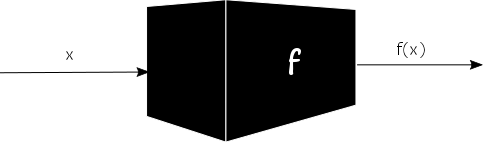
\includegraphics[height=5cm]{pic/blackbox.png}
\end{figure}

Запросы к черному ящику можно генерировать либо случайным образом, либо основываясь на результаты предыдущих запросов. В лучшем случае, алгоритм может не запрашивать уже запрошенное повторно.

\chapterconclusion

В данной главе была поставлена решаемая задача, а так же ожидаемые к ней подходы в модели несмещенной blaсk-box сложности. Также были описаны уже существующие решения и оценки их работы, что 
демонстрирует научную новизну представленной работы. 

\newcommand{\cupdot}{\mathbin{\mathaccent\cdot\cup}}

\chapter{Верхние и нижние оценки}
\label{chapter3}

%По-моему, повтор первой главы. 
%И вообще, не здесь нужно говорить об оценках, а во второй главе. Зедсь чуть-чуть расписать про операторы и погнать примеры.

\section{Оценка сложности алгоритмов с несмещенными операторами}

Особый интерес в рамках данной работы над задачей Needle представляет собой класс несмещенных алгоритмов арностей k. Под несмещенными алгоритмами (произвольной арности) понимаются алгоритмы
следующего вида:

\begin{itemize}
   \item Запрос $Q_1$ - запрос, сгенерированный случайным образом.
   \item Запрос $Q_{i+1}$ - реализация случайной величины, такой что:
    $ \forall z: p(Q_{i+1} | & Q_1, ... Q_i, A_1, ... A_i) =  
     p(Q_{i+1} \oplus z | Q_1 \oplus z, ..., Q_i \oplus z, A_1, ..., A_i) $
    \begin{align*}
    $ \forall perm():$  p(Q_{i+1} | Q_1, ..., & Q_i, A_1, ..., A_i) = \\ &= p(perm(Q_{i+1}) |perm(Q_1), ..., perm(Q_i), A_1, ... A_i) 
    \end{align}
  \end{itemize}
         
Иными словами, функция, генерирующая запрос, не меняется, если индексы
всех битовых строк переставить одинаковым образом, или если все битовые строки поксорить с константой. 

Алгоритм арности k: случайная величина, генерирующая $Q_{i+1}$ рандомизировано выбирает не более k различных индексов $H_j$ из $[1; i]$ и генерирует $Q_{i+1}$ используя только $Q_{H_1}, ..., Q_{H_K}, A_{H_1}, ... A_{H_K}$ Разумеется, при этом она обязана быть несмещенной.

Для примера, унарный (k = 1) алгоритм может следующий запрос сделать либо совсем случайным, либо взять какой-то из предыдущих запросов и применить к нему унарный несмещенный "оператор мутации". Унарные операторы мутации, как нетрудно показать, имеют вид "выбрать из некоторого распределения число X (от 0 до n), выбрать случайным образом X различных битовых индексов и перевернуть биты на каждом из этих индексов".

Обсобый интерес представляют собой несмещенные операторы арностей k = 1, 2, 3, а соответственно и несмещенные алгоритмы, работающие с данными операторами.

В рамках рассматриваемой black-box сложности, получение оценок на сложность работы алгоритмов состоит в нахождение верхних и нижних оценок. Верхние оценки сложности представлют собой оценку работы некоторого алгоритма, который решает задачу. При этом алгоритм не обязательно является эволюционным. Верхняя оценка - оценка любого алгоритма, решающего задачу в принципе. 

Нижние оценки представляются гораздо сложнее. Чаще всего для получения нижних оценок используются информационно-теоретические оценки, что гораздо сложнее, чем получение верхних оценок. Зачастую подсчет сводится к нахождению общего вида всех алгоритмов данного класса, нахождению вещественнозначных параметров, однозначное определяющих работу алгоритма, построению выражения, зависящего от указанных параметров и определяющего математическое ожидание времени работы алгоритма, и, наконец, минимизации времени работы. При отсутствии аналитического решения, задача решается численным моделированием.   

\subsection{Тернарный алгоритм}
\label{ternary}

%бедно и непонятно, исправить обязательно. Может подумать о картинке в пример, дабы было нагляднее. 


В качеcтве операторов для данного алгоритма введем следующие несмещенные операторы: 
\begin{itemize}
   \item $flipOne(a)$ - изменение одного бита
   \item $flip'(a, b)$ - изменить один бит из совпадающего суффикса
   \item $xor3(a,b,c)$ - оператор исключающего ИЛИ для трех векторов 
\end{itemize}

(вставить формальное доказательство, что xor3 -> несмещенный)

Тогда рассмотрим следующий алгоритм: 
\begin{algorithm}[H]
\caption{Тернарный алгоритм}\label{lst1}
\begin{algorithmic}
        \State $q_0$ \leftarrow $\textrm{random}$ \\
        \State $s_1$ \leftarrow $flipOne(q_0)$
		\While{true}
	        \State $s_2$ \leftarrow $flip'(q_0, s_1)$
            \State $t_2$ \leftarrow $xor3(q_0,s_1,s_2)$
            \State $s_3$ \leftarrow $flip'(q_0, t_2)$
            \State $t_3$ \leftarrow $xor3(q_0,s_2,s_3)$
            \State ...
		\EndWhile
\end{algorithmic}
\end{algorithm}

Таким образом формируется полное пространство поиска: 
\begin{example}
Пример генерации пространства для q_0 = [000...000]  \\
\end{example}

\begin{figure}[H]
%\caption{Пример генерации множества поиска для q0}\label{fig2}
    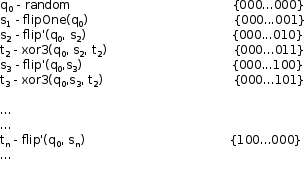
\includegraphics[height=7cm]{ITMO/pic/tern0.png}
\end{figure}


%Размазано и непонятно. Переписать точно.
Таким образом пошагово генерируется все множество поиска без повторов. Сложность такого алгоритма равняется O($\frac{2^n + 1}{2}$), что равняется времени перебора всех векторов без повторов. Таким образом, верхняя и нижняя оценки сложности алгоритма совпадают. 


%Что-то вроде примера 
Рассмотрим класс некоторых задач, таких что экземпляром данной задачи является битовая строка из пространства поиска, размера $2^n$ от длины строки n. При этом у задачи существует единственный глобальный оптимум (при этом  наличие других оптимумов не важно). К таким задачам относится, например, OneMax.

Задачи данного класса должны имееть примерно такой тип:
$$P = \{..2^n \textrm{instanses with bitwise} ... \}$$

Пусть существует оптимальный детерминированный алгоритм, который в среднем по всем экзеплярам выдает время работы T, при этом алгоритм не является black-box алгоритмом. 

Пусть $q_0$ - рандомизированный вектор, подающийся на вход алгоритму.

Тогда дерево решений данного алгоритма выглядит так: 

\begin{figure}[H]
\caption{Дерево решений детерминированного алгоритма}\label{fig2}
    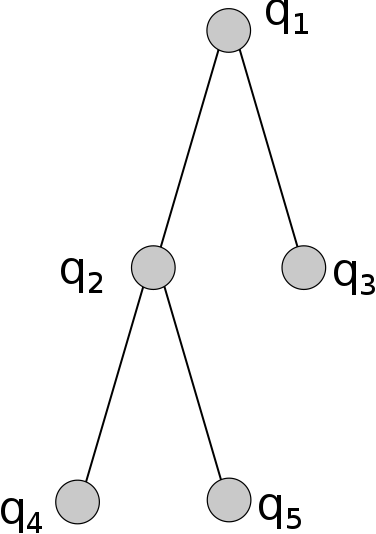
\includegraphics[height=5cm]{ITMO/pic/graph1.png}
\end{figure}

Возьмем произвольный вектор z и проксорим его с каждым решением из приведенного выше дерева. Таким образом все равно получится оптимальный детерминированны алгоритм, решающий данную задачу, но выглядеть он будет уже иначе, допустим, так: 

\begin{figure}[H]
\caption{Дерево решений другого оптимального алгоритма}\label{fig2}
    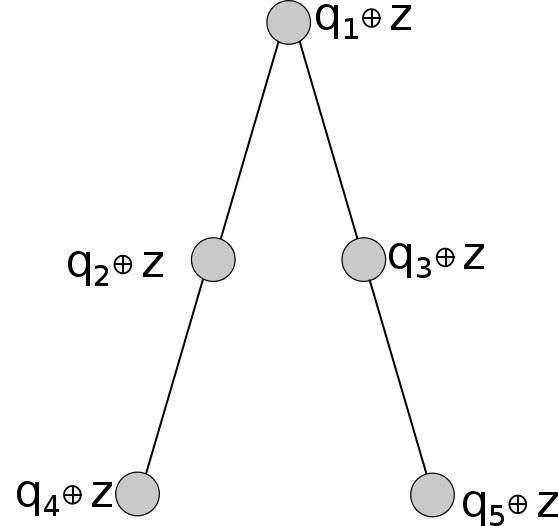
\includegraphics[height=5cm]{ITMO/pic/graph2.png}
\end{figure}

Тогда моделизируем процесс. 
$q_0$ - так и остается рандомизированным вектором.
Исходя из дерева решений, известно, что переход в дереве от $q_1 \to q_2$ является не более чем изменением одного бита. 

Так как при моделировании аллгоритма с тернарным оператором мы можем сгенерировать множество векторов, показанное в примере 3, то мы умеем получать переходы при изменении от одного бита к другому. 

Тогда z больше не просто случайный вектор, а $z = q_0 \oplus q_1 $, что, таким образом, и будет являться переходом $q_1 \to q_2$ в дереве решений. А так как при применения $\oplus$ к вершине изначального дерева, так же получается детерминированный алгоритм, то учитывая построение множества, тогда несмщенный black-box алгоритм будет работать за $\leq(n + 1)T$



\subsection{Бинарный алгоритм}
\label{binary}

Основная идея алгоритма с несмещенныи бинарными операторами заключается в следующих двух этапах: формирование независимых уникальных строк без использования операторов 
с помощью примитивных пошаговых пеобразований и формирование всего оставшегося множества поиска, стараясь минимизировать количество повторений. 

Рассмотрим первый этап: создание множества уникальных строк.

Введем следующее: пусть ${I_0}^1 = \{1,\ldots, n\}$ - множество индексов в искомом экземпляре, поданном на вход задаче. 

Каждый этап выглядит следующим образом: 
\begin{align*}
& L_i = \langle \mathcal{I}_i = \{{\mathcal{I}_{i}}^{1},....{\mathcal{I}_{i}}^{k};\}; \:\: \textrm{где}  \cupdot_{a = 1..k_i} {I_i}^a = \{ 1..n \}; \\
& S_i = \{ {S_i}^1, ... {S_i}^{m_i}, \}, \textrm{где}  \\ 
&{s_i}^j = b_1..b_{k_i}, b_k = \{ 0..1  \}  \Longleftrightarrow b_1 \textrm{ на индексах } {I_{i}}^1, \\ & \:\:\:\:\:\:\:\:\:\:\:\:\:\:\:\:\:\:\:\:\:\:\:\:\:\:\:\:\:\:\:\:\:\:\:\:\:\:\:\:\:\:\:\:\:\:\:\:\:\:\:\:\:\:\:\: b_e \textrm{ на индексах } {I_{i}}^e\\
 \rangle
\end{align*}

Таким образом, самый первый уровень будет выглядеть так: 
$$L_0 = \langle \{\{ 1...n \}\}, \{0\} \rangle.$$

Каждый последующий уровень $L_i$ можно получить двумя способами: 
\begin{itemize}
   \item Разделить одно из множеств индексов пополам: $ \mathcal{{I}_i}^j \to \{\mathcal{{I}_{i+1}}^j, \mathcal{{I}_{i+1}}^{k_i+1}\} $, где $j \in [1..k_i]$;
   \item Преобразование строк с помощью операций, не разрезающих множества индексов.
\end{itemize}

При разделении множества индексов, уже имеющиеся строки преобразуются удваиванием бита, находящегося на позиции, множество индексов которого разделилось.
Таким образом гарантируется, что следующая полученная строка будет уникальна.

К неразделяющим множества индексов операциям относятся следующие оперции, которые можно применять попарно ко всем полученным векторам: 
переворот несовпадающих бит, переворот совпадающих бит, поворот совпадающих и несовпадающих бит. 
Нетрудно заметить, что данные операции являются несмещенными, так как не ориентируются на положение бита, а только на совпадение в этой же позиции с битом второго вектора. 

Таким образом генерируются маски последуюших строк. 

\begin{example}
Пример генерации строк для вектора размера $n = 6$ \\
    I = \{1, 2, 3,4,5,6\} \:\: S = \{0\} \\
    I = \{1, 2, 3,4,5,6\}  \:\: S = \{0, 1\} \\
    I = \{1, 2, 3\}, \{4,5,6\} \:\: S = \{00, 11\} \\
    I = \{1, 2, 3\}, \{4,5,6\} \:\: S = \{00, 11, 01, 10\} \\
    I = \{1, 2\}, \{3\}, \{4,5,6\} \:\: S = \{000, 111, 001, 110\} \\
    I = \{1, 2\}, \{3\}, \{4,5,6\} \:\: S = \{000, 111, 001, 110, 011, 100\} \\
    ...
\end{example}

В силу перечисленных выше изменений векторов, из полученных масок и индексов генерируется некоторое число уникальных строк. 
Так как таким путем нельзя получить полное множество поиска, оставшиеся строки генерируются следующим образом:  

\begin{algorithm}[!h]
\caption{Black-box алгоритм в несмещенной модели}\label{lst1}
\begin{algorithmic}
		\For{$t = S_1,S_2,S_3,...,S_\phi$ }
	    \State choose $i \in [1 : \phi] $
	    \State choose $j \in [1 : \phi] $
	    \State $e \leftarrow$ same bits in $\{S_i, S_j\}$
	    \State $d \leftarrow$ different bits in $\{S_i, S_j\}$
	    \State choose $k \in [1 : e] $
	    \State choose $l \in [1 : e] $
	    \State add to $T_{ijkl}$ - множество строк, генерируемых из $S_i$ и $S_j$ путем инвертирования k совпадающих и l различающихся бит в $S_i$
		\EndFor
\end{algorithmic}
\end{algorithm}

Таким образом генерируется множество конструкций, содержащих $T_{ijkl}$:   $\mathbb{T} = \{ T_{ijkl} \}$.
    
    \begin{math}
        \mathbb{T'} \subseteq \mathbb{T} : 
                   \left\{  
           \begin{array}{rcl}  
            \forall t, u \in \mathbb{T'} \quad t \cap u = \varnothing \\  
              \cup = {\{0, 1 \}}^n \setminus \{S_1...S_{\phi}\} \\  
           \end{array}   
           \right.
    \end{math}


Таким образом, мы получаем область поиска с некоторыми повторами, что немного, но улучшает работу. С увеличением длины подаваемого на вход вектора, увеличивается количество повторов.
На рисунке~\ref{fig1} показано распределение множества $T'$ для $n = 6$. При этом размер множества составлял 4097 строк.

\begin{figure}[H]
\centering
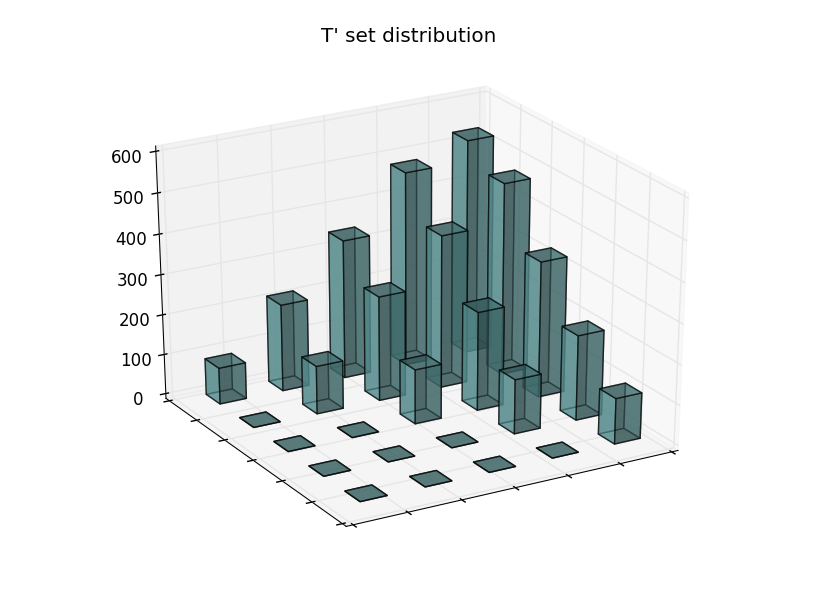
\includegraphics[height=10cm]{pic/fig6_n.png}
\caption{Распределение для n = 6}\label{fig1}
\end{figure}

Для улучшения результатов, применим к получившемся множествам некоторые преобразования. Сравним некоторые множества $T_{ijkl}$ между собой на наличие повторяющихся строк следующим образом: 

\begin{algorithm}[H]
\caption{Фильтрация повторяющихся множеств}\label{lst1}
\begin{algorithmic}
        \State Создаем неориентированный граф, вершины которого - множества $T_{ijkl}$ 
        \For{$i = 0, 1, \ldots, \mathbb{T}.same$}
	        \For{$j = 0, 1, \ldots, \mathbb{T}.diff$}
    	        \State Если между двумя множествами нет совпадающих строк, то соединяем данные вершины ребром.   
	        \EndFor
	    \EndFor
	    \State Дальнейшая задача сводится к поиску максимальной клики в графе.
\end{algorithmic}
\end{algorithm} 

По результатам работы алгоритма были рассмотрены два варианта действий. 
Рассмотрим несколько максимальных полученных клик, множества которых покрывают все пространство поиска. Экспериментально было установлено, что в результате нахождения клик
было отброшено достаточно большое количество повторов и итоговое отфильтрованное множество содержало и меньше векторов, и меньше повторов. 
Рассматривалось распределение для $n = 6$. В результате перебора всех пар значений было получено 4097 строк. По результатам фильтрации и поиска непересекающихся множеств осталось 306 векторов.
На рисунке~\ref{fig2} показано распределение при объединении двух клик. 

\begin{figure}[H]
\centering
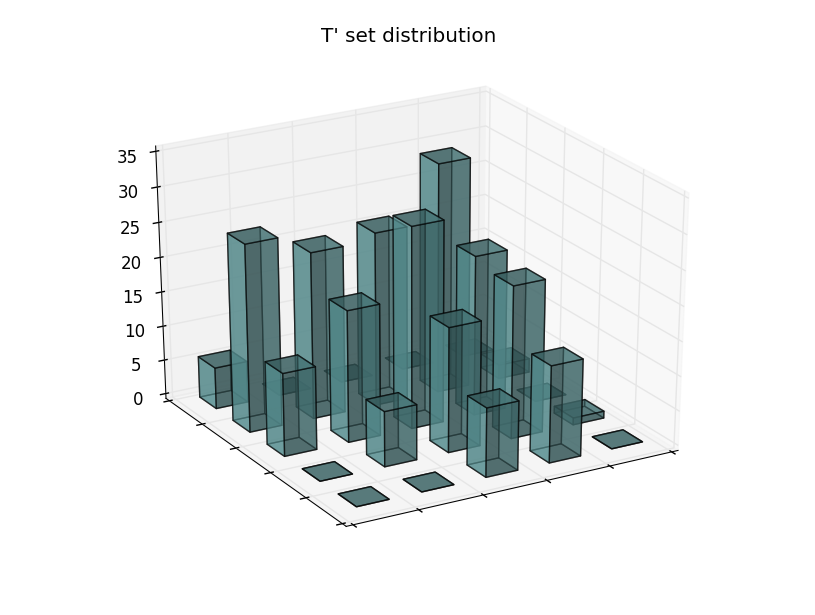
\includegraphics[height=10cm]{pic/fig6_mod2.png}
\caption{Выборка непересекающихся множеств для $n = 6$, подход 1}\label{fig2}
\end{figure}

Второй подход заключается

В результате выполнения алгоритма, гарантируется, что на выходе получится множество строк без повторов. 
При объединении полученного множества $T$ и получившихся на первом этапе строк, итоговое множетсво не превышает $2\cdot2^n$. 
Таким образом получается следующее распределение для $n = 6$, при этом размер множества составлял 124 строки. 

\begin{figure}[H]
\centering
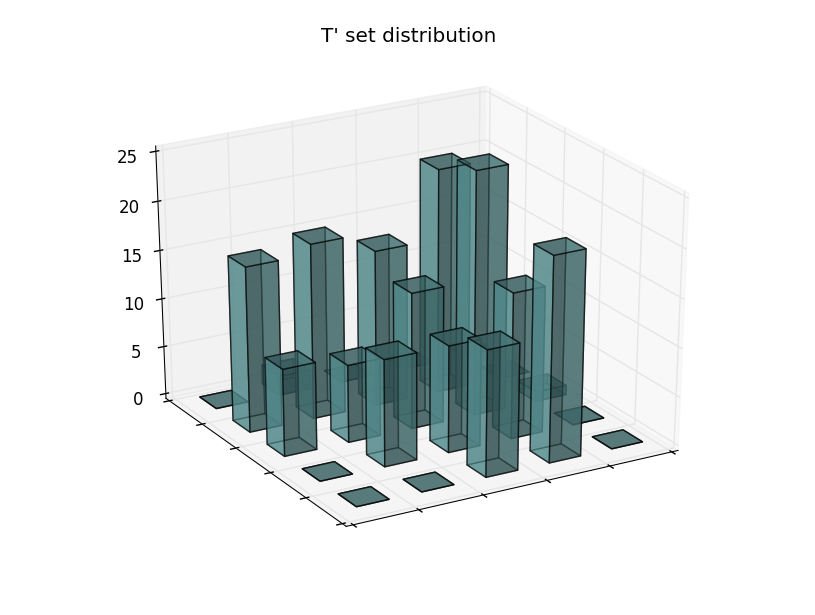
\includegraphics[height=10cm]{pic/fig6_mod3.png}
\caption{Выборка непересекающихся множеств для n = 6, подход 2}\label{fig2}
\end{figure}

В результате вызыва алгоритма для особей маленьких размеров, было замечено, что размер множества с повторами от увеличения размера особи растет экспоненциально. В таблице представлены результаты запуска для некоторых векторов:

\begin{table}[!h]
\caption{Результаты работы алгоритма с бинарными операторами}\label{tab3:apx}
\centering
\begin{tabu}{|*{6}{X[c]|}}\hline
n & 3 & 4 & 5 & 6 & 7  \\
\hline
set size & 8 & 16 & 32 & 64 & 128 \\
\hline
{T' size} & 64 & 256 & 1024 & 4096 & 16384  \\
\hline
{mod(T') size} & 11 & 36 & 73 & 144 & 302  \\
\hline
\end{tabu}
\end{table}

Ниже на рисунке~\ref{fig3} приводится диаграмма по количеству полученных совпавших строк и количеству оставшихся после модификации (берется лучшее значение).

\begin{figure}[H]
\centering
\caption{Выборка непересекающихся множеств для $n = 6$, подход 2}\label{fig3}
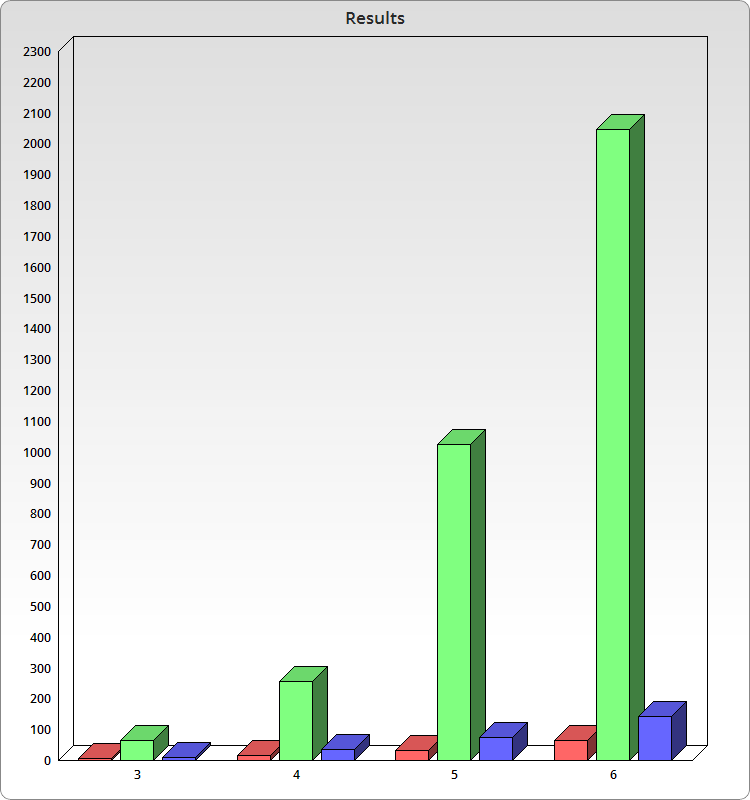
\includegraphics[height=10cm]{pic/res_bin.png}
\end{figure}


\subsection{Унарный алгоритм}
\label{unary}

%описание оператора и принципа
В силу того, что унарный несмещенный оператор может изменять только один случайный бит в векторе, в модели генетических алгоритмов он представляет собой оператор мутации. 

(Не хватает немного)

Разобъем все пространство поиска на некоторые классы векторов, где каждый шаг - это расстояние между первоначальным вектором и векторами этого множетсва, то есть, количество отличающихся бит. Классы будут генерироваться слеующим образом: 
\begin{itemize}
   \item $q_0$ $\leftarrow$ random
   \item $D_1$ - класс решений, отличающихся от первоначальной особи на 1 бит, размер множества n
   \item $D_2$ - размер ${n}\choose{2}$
   \item $D_3$ ...
   \item ...
   \item $D_{n-1}$ - размер ${n}\choose{n - 1}$ = n
   \item $D_n$ - размер 1, \bar{q_0}
\end{itemize} 


\newtheorem{theorem}{Теорема}
\begin{myth}
Даны непересекающиеся множества $S_1, ... S_k$ размеров $n_1 ... n_k$.
В одном из множеств находится элемент x. Утверждается, что в этой постановке при отсутствии другой информации, оптимизационный алгоритм выглядит так: 
\begin{algorithm}[H]
\caption{Унарный алгоритм}\label{lst1}
\begin{algorithmic}
        \For{i = 0, ... , k}
	    \State Храним $t_1 ... t_k$ - сколько запросов было сделано к соответствующему множеству
	    \State На определенном шаге вычисляем $E[z_i] = (\frac{n_i - 1}{n_i})^{t_i}$
	    \State Выбираем множество i c максимальным $E[z_i]$ и делаем запрос к этому множеству.
	    \EndFor
\end{algorithmic}
\end{algorithm}
\end{myth}
\begin{proof}
    Пусть мы знаем, сколько уникальных элементов $u_1...u_k$ было запрошено из каждого множества. Известно что количество элементов будет меньше или равно числу запросов к множеству. ($u_i \leq t_i$). 
    
    Пусть x - искомый экземпляр данной задачи, находится соответственно в одном из множеств. Предположим, что элемент x раньше не возвращался из запросов (так как при возвращении искомого элемента функция бы завершилась).
    
    
    $P_i$ = [вероятность, что $x$ лежит в $i$] = $\frac{t_i - u_i}{\sum_{j}{t_j - u_j}}$ 
    
    $p_i$ = [вероятность, что на запросе к i вернут k] = $\frac{1}{n_i} \cdot P_i$ = $\frac{n_i - u_i}{\sum_{j}{t_j - u_j}}$
    
    Так как $u_i$ - величина переменная а каждом шаге, можем посчитать матожидание в таком формате: $u_i \sim E(u_i(n_i, t_i))$
    
    До запроса было x уникальных запросов, после запроса будет: $$x + \frac{n - x}{n} = 1 + x \cdot (1 - \frac{1}{n_i})$$ 
    
    Таким образом: $E[u(n_i, t_i)] = 1 + E[u_i(n_i, t_{i} - 1)] \cdot (1 - \frac{1}{n_i})$
    
    Для $ t_i = 0 \to 0 $ - база индукции.
    
    Рассмотрим переход: 
    $E[u(n_i, t_i)]$ = $\frac{{n_i}^{ti} - {(n_i - 1)}^{ti}}{{n_i}^{t_i - 1}}$  = 1 + $[ \frac{{n_i}^{ti} - {(n_i - 1)}^{t_i}}{{n_i}^{t_i}} ] \cdot (\frac{1}{n_i})$ = $ \frac{{n_i}^{ti + 1} - {(n_i - 1)}^{t_i + 1}}{{n_i}^{t_i}} $ 
    
    Таким образом мы получаем значение, равное количеству строк на следующем шагу, а значит, теорема доказана.

\end{proof}

%здесь будет вставка от Дена для увеличения объема работы. Не знаю, пригодится ли дальше это, но пока пусть будет.

(доделать доказательство, доделать разбор вероятностей по классам)




\chapterconclusion

В этой главе представлены алгоритмы решения задачи Needle, использующие несмещенные операторы, а так же информационно-теоретические оценки времени работы данных алгоритмов. Были рассмотрены унарные, бинарные и тернарные несмещенные операторы. 
Основной вывод главы заключается в получении верхних оценок на операторы арностей k = 1, 2, 3, а так же получение того, что нижняя и верхняя оценка работы тернарного алгоритма совпадают.











\startconclusionpage

Результатом данной работы являются достаточно точные оценки на работу несмещенных операторов для несмещенной black-box сложности.
Были установлены верхняя и нижняя оценка на работу тернарного оператора. Также было установлено, что необходимости рассматривать операторы с большей арностью нет, то есть при $k = 3$ достигается 
оптимальное значение. Тернарный оператор можно применять к некоторым классам задач, так как алгоритм, использующий таковые, работает не хуже оптимальных детерминированных алгоритмов.  

Также были проделаны исследования бинарного и унарного операторов. Были установлены некоторые ограничения на время работы бинарного оператора, а так же предложен алгоритм работы с бинарным оператором. 
Более точные оценки еще предстоит получить.

Был разработан алгоритм работы унарного оператора, а так же получение всего пространства поиска для алгоритма, использующего таковой. 
Результатом исследования унарного оператора стала верхняя оценка на количество запросов данного алгоритма к пространству поиска. 

Полученные оценки явно показывают, что задачу Needle можно разрешить быстрее, чем простым перебором. Идеи, использованные в разработанных алгоритмах, могут быть использованы в будущем для других задач, 
к примеру, к обходу плато, которые встречаются во многих оптимизационных задачах.

Среди открытых вопросов остаются нижние оценки для бинарных и унарных операторов.


%% Обратите внимание на heading. Без него тоже работает, но название будет другим.
%\printmainbibliography

\begin{thebibliography}{9}
\bibitem{1} Per Kristian Lehre, Carsten Witt. \textit{Black-box search by unbiased variation}. In Proceedings of Genetic and Evolutionary Computation Conference (GECCO’ 10), p. 1441– 1448. ACM, 2010.
%\bibitem{einstein} Albert Einstein. \textit{Zur Elektrodynamik %bewegter K{\"o}rper}. (German) [\textit{On the electrodynamics of %moving bodies}]. Annalen der Physik, 322(10):891–921, 1905.

%\bibitem{knuthwebsite} Knuth: Computers and Typesetting,\\\texttt{http://www-cs-faculty.stanford.edu/\~{}uno/abcde.html}

\bibitem{2} Stefan Droste, Thomas Jansen, and Ingo Wegener. \textit{Upper and lower bounds for randomized search heuristics in black-box optimization}. Theory of Computing Systems, 39:525–544, 2006.

\bibitem{3} B. Doerr and C. Winzen. \textit{Ranking-based black-box complexity}. Algorithmica. To appear. DOI: 10.1007/s00453-012-9684-9б 2012. \\\texttt{http://arxiv.org/pdf/1102.1140.pdf}

\bibitem{4} B. Doerr and C. Winzen. \textitReducing the arity in unbiased black-box complexity}. Theor. Comput. Sci., 545:108–121, 2014 \\\texttt{http://arxiv.org/pdf/1203.4111.pdf}

\bibitem{5} Andrew Chi-Chih Yao. \textit{Upper and lower bounds for randomized search heuristics in black-box optimization}. Probabilistic computations: Toward a unified measure of complexity (extended abstract). In FOCS, pages 222–227. IEEE Computer Society, 1977

\bibitem{6} A. J. Ramirez, D. B. Knoester, B. H. Cheng, and P. K. Mckinley. \textit{Plato: a genetic algorithm approach to run-time reconfiguration in autonomic computing systems}. Cluster Computing, 14:229–244, 2011

\bibitem{7} T. Jansen and I. Wegener. \textit{Evolutionary algorithms — how to cope with plateaus of constant fitness and when to reject strings of the same fitness}. In IEEE Trans. on Evolutionary Computation, volume 5, pages 589–599, 2001.

\bibitem{8} Benjamin Doerr, Carola Doerr and Timo Kötzing. \textit{Unbiased Black-Box Complexities of Jump Functions}. Evolutionary Computation, volume 23 Issue 4, 2015 Pages 641-670 

\bibitem{9} Buzdalov, M., Kever, M., and Doerr, B. \textit{Upper and lower bounds on unrestricted black-box complexity of $jump_{n,l}$}. In Evolutionary Computation in Combinatorial Optimization, pp. 209–221. Lecture Notes in Computer Science, Vol. 9026.

\bibitem{10} Benjamin Doerr, Timo Kötzing  and Carola Winzen. \textit{Too fast unbiased black-box algorithms}. In Proc. of GECCO (Genetic and evolutionary computation), pages 2043–2050, 2011.

\bibitem{11} Benjamin Doerr, Carola Doerr and Franziska Ebel. \textit{From black-box complexity to designing new genetic algorithms}. Theoretical Computer Science archive Volume 567 Issue C, 2015 Pages 87-104

\bibitem{12} Doerr, B., Doerr, C., Ebel, F. \textit{Lessons from the black-box: fast crossover-based genetic algorithms}. In Proceedings of Genetic and Evolutionary Computation Conference. pp. 781–788 (2014)

\bibitem{13} Doerr, B.\textit{ Analyzing randomized search heuristics: Tools from probability theory}. In A. Auger and B. Doerr (Eds.), Theory of randomized search heuristics, pp. 1–20 (2011)

\end{document}
